\documentclass[a4paper]{article}
\usepackage{amsfonts}
\usepackage{a4wide,times}
\usepackage[english]{babel}
\usepackage{graphicx}
\usepackage{listings}
\lstset{language=Java,
  numberstyle=\footnotesize,
  basicstyle=\footnotesize,
  numbers= left,
  stepnumber=1,
  tabsize=2,
  frame=shadowbox,
  breaklines=true
}


\begin{document}

\title{Net-computing\\
Architectural design document
}

\date{9.3.2018}

\author{Peri Rahamin (s2683423),\\
Jits Schilperoort (s2788659),\\
Twan Schoonen (s2756978)
}




\maketitle
\section*{Smart car on demand}
\subsection*{Project description}
Smart car on demand is the name of our project idea to have self-driving cars drive through the city, and get ordered by customers who wish to go somewhere using this service. The order is done by a costumer logging in to a mobile application, and select their destination and number of passengers.

The request has the user's location saved, is sent to the car canter, that selects the nearest car that can handle the request. Payment is done via money that is saved in the app account (top up is required beforehand). Requests are handled in queue order (first order-first served).

The car arrives to the costumer(s) and takes them to their destination. Selecting a car and planning routes are handled by Artificial Intelligence systems that is able to compute the shortest route. The AI also allows the automated cars to drive without human intervention.

Cars are able to communicate with other cars for request handling, such as big order that one car alone is not enough to handle, and requesting another car to reach a costumer. This type of communication can normally be handled by a car center, but for the sake of the project we will implement it this way.
\\\\Since this is a big project, we will not implement all of the features, but only those relevant for this course. This list specifies the different elements of the system, with an explanation of why we decided to implement or not implement it:
\begin{itemize}
    \item \textbf{Mobile application:} Each costumer that is interested in getting a car to drive them uses a mobile app to make the order. A working app with an user friendly GUI is irrelevant for this course, so we decided to have some data structure that represents a user and has location and number of people who want to use the service instead.
    \item \textbf{AI:} The automated driving cars should know how to drive on roads without the help of humans. The AI of the car should follow the law and consider other cars (agents) or people crossing the road in its surrounding. This part is obviously too much to implement, and since it is also irrelevant to this course, we decided to assume the AI works.
    \item \textbf{Shortest distance algorithm:} We want the car to find the best route to reach its costumer, considering traffic and other parameters (such as construction that blocks the road). The algorithm helps deciding which car is most suitable to get to a costumer, in case there are few of them in different parts of the city. To make this work we need live data, so for this project, we only send messages with datasets we made ourselves, and leave out the complicated calculations.
    \item \textbf{Wireless communication:} The cars should communicate with each other, deciding which costumer to get to first. We will implement this part of the system, that covers socket and message queuing.
\end{itemize}

\subsection*{Project requirements}
%TODO: improve list
The requirements that are implemented in this project are listed as follows:
\begin{itemize}
    \item \textbf{Socket:} used for car control.
    \item \textbf{Message queuing:} the requests made by the mobile application are queued until an available car pops a request in order to handle the costumer.
    \item \textbf{Web services (REST):} the mobile app communicates with the cars thus making use of web services.
\end{itemize}

\subsection*{Cars communication}
When a customer's request is received, the cars communicate with each other in order to decide which of them should pick up the customer. This decision is based on both the availability of the cars and the distance of the car from the customer.

Whenever a change is made in the system (e.g. a customer is picked up), it is preferable that the cars are evenly distributed around the area while taking into account areas with many requests. For this reason it is necessary that cars communicate with each other in order to figure out what their new path should be.
%TODO: more elaborated description of what information the cars share
\subsection*{Component diagram}
%TODO

\subsection*{Class diagram}
%TODO

\subsection*{Sequence diagrams}
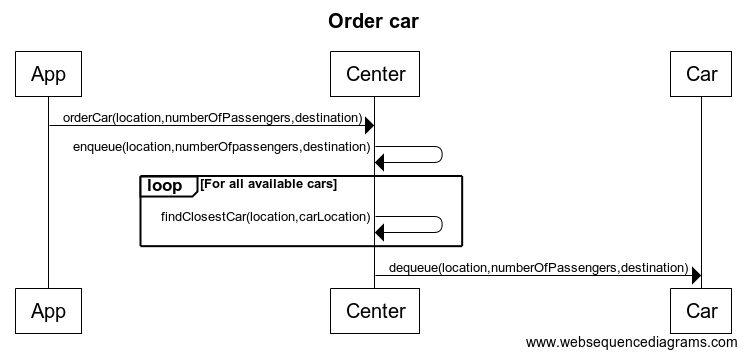
\includegraphics[width=1\textwidth]{sd1.png}
%TODO: car communication diagram-in which cases does it happen?

\subsection*{Star vs P2P topology}
\textbf{Star topology:} This method is implemented by the mobile application. A central node holds all requests for a car in a queue. The central node pops requests and sends them to a free car.
\\\textbf{P2P topology:} This method is used in cars communication between themselves. Passing requests from one car to another if it is found to be a better option.
%TODO: elaborated description

\end{document}

